\subsubsection*{ --- Testing Results}
Two methods are used to test and validate system's performance. First, an arbitrary force is applied to the handle, after user terminates the program, both force readings and velocities are exported to MATLAB file for validation. In this case, input mode 1, which uses actual reading as force input for Simulink model, is used. A sample plot of the simulated results vs. actual velocity can be found in Appendix {{\color{red}\ *}}. Error between recorded and reference speed is also calculated by taking average of error at each time stamp and it is found to be in the scale of $10^{-6}$. 

The second method utilizes a pulley and weight system. The mechanism simulates a constant force input on the handle. Same weight is used in all tests to keep input force a constant. Equivalent force applied on the handle is approximately 3N. The 3N force is also used in simulation as a step input. Three sets of tests are run using this method and each set contains three cases. In each set, only one virtual parameter is adjusted. 

As shown in Figure \ref{fig:MChange}, spring constant is eliminated for clarity of the test, damping is kept at a constant of 50 N*s/m and mass ranges from 5kg to 40kg. In each plot, green lines represent the actual velocity recorded by C, red and blue lines represent reference velocity calculated by C and Simulink respectively. From left to right, mass is 5kg, 20kg and 40kg for each line. The lines represent different acceleration due to change in mass.  Since all three cases utilize the same input force and damping constant, their steady state speed all converge to the same point which is expected from 
\begin{equation}
F=B*v
\end{equation}
\begin{figure}[H]
\centering
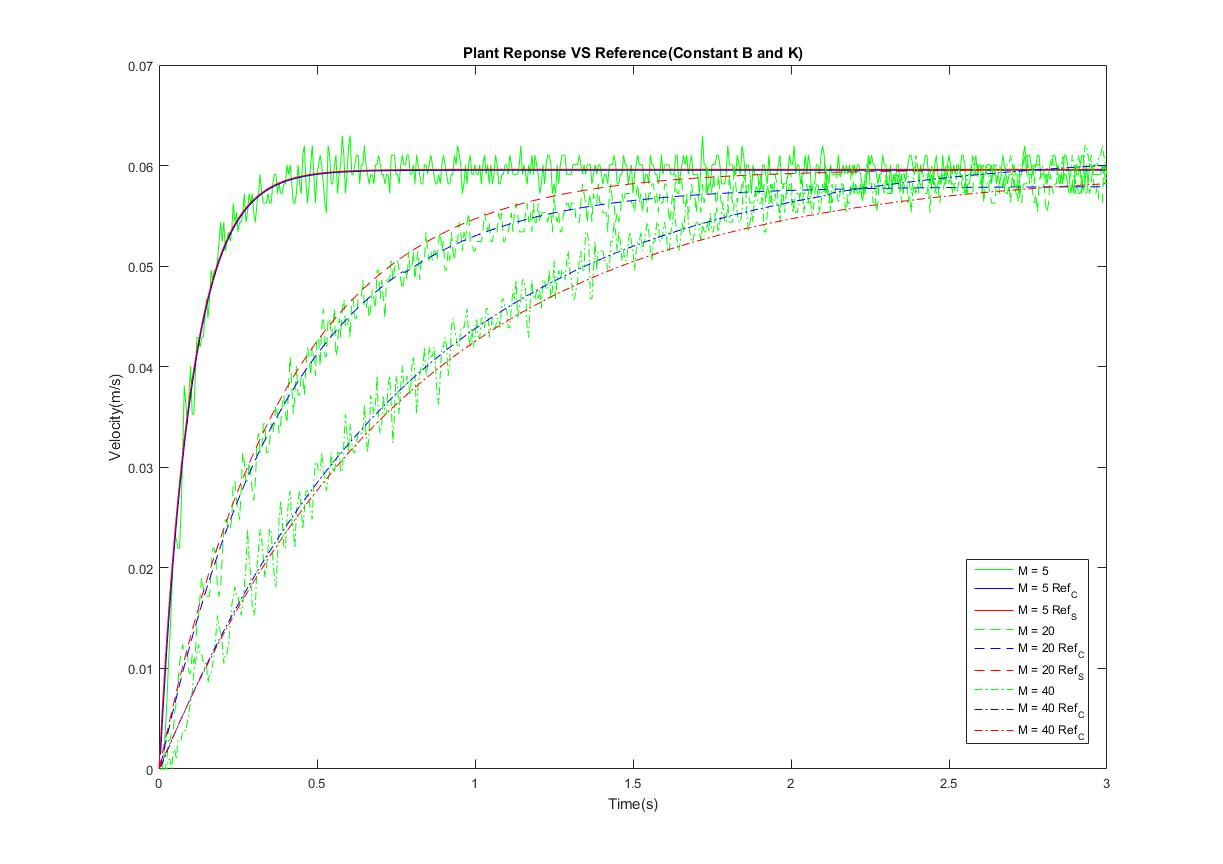
\includegraphics[width=1\linewidth]{Images/MChange}
\caption{Actual and Reference Velocity for Constant Damping with Adjusted Mass System}
\label{fig:MChange}
\end{figure}

Shown in Figure \ref{fig:BChange} is a same virtual mass with different damping constants applied on it. For all cases, mass is kept at 10kg whereas damping ranges from 25N*s/m to 100N*s/m. The steady state speed now changes due to the change in damping constant, which can be verified using equation mentioned in previous paragraph. From top to bottom, damping constant is 25N*s/m, 50 N*s/m and 100N*s/m for each case. 
\begin{figure}[H]
\centering
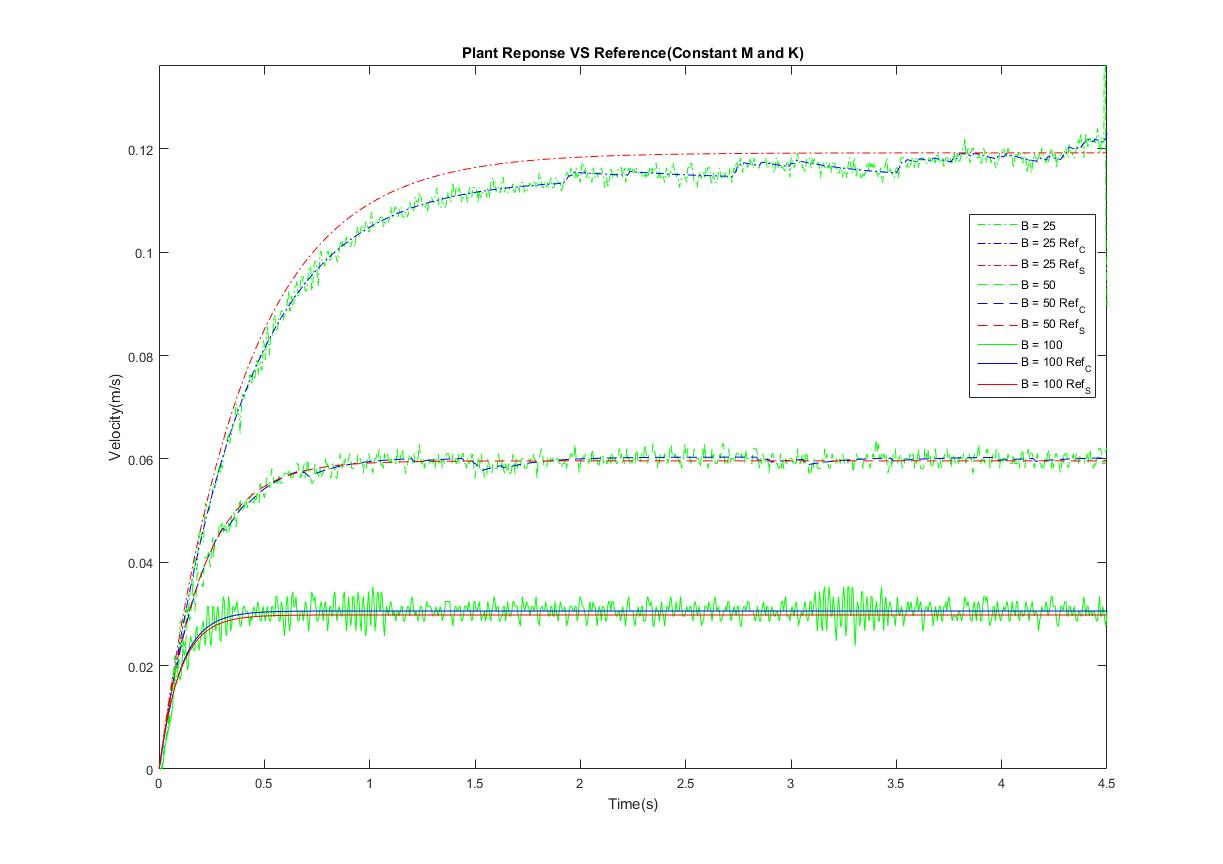
\includegraphics[width=1\linewidth]{Images/BChange}
\caption{Actual and Reference Velocity for Constant Mass with Adjusted Damping System}
\label{fig:BChange}
\end{figure}

Lastly, shown in Figure \ref{fig:KChange}, both mass and damping are kept constant and spring is the only variable. From top to bottom, spring constant increases from 0 to 20N/m. The change in spring constant resulted in a different deceleration rate for the systems. 
\begin{figure}[H]
\centering
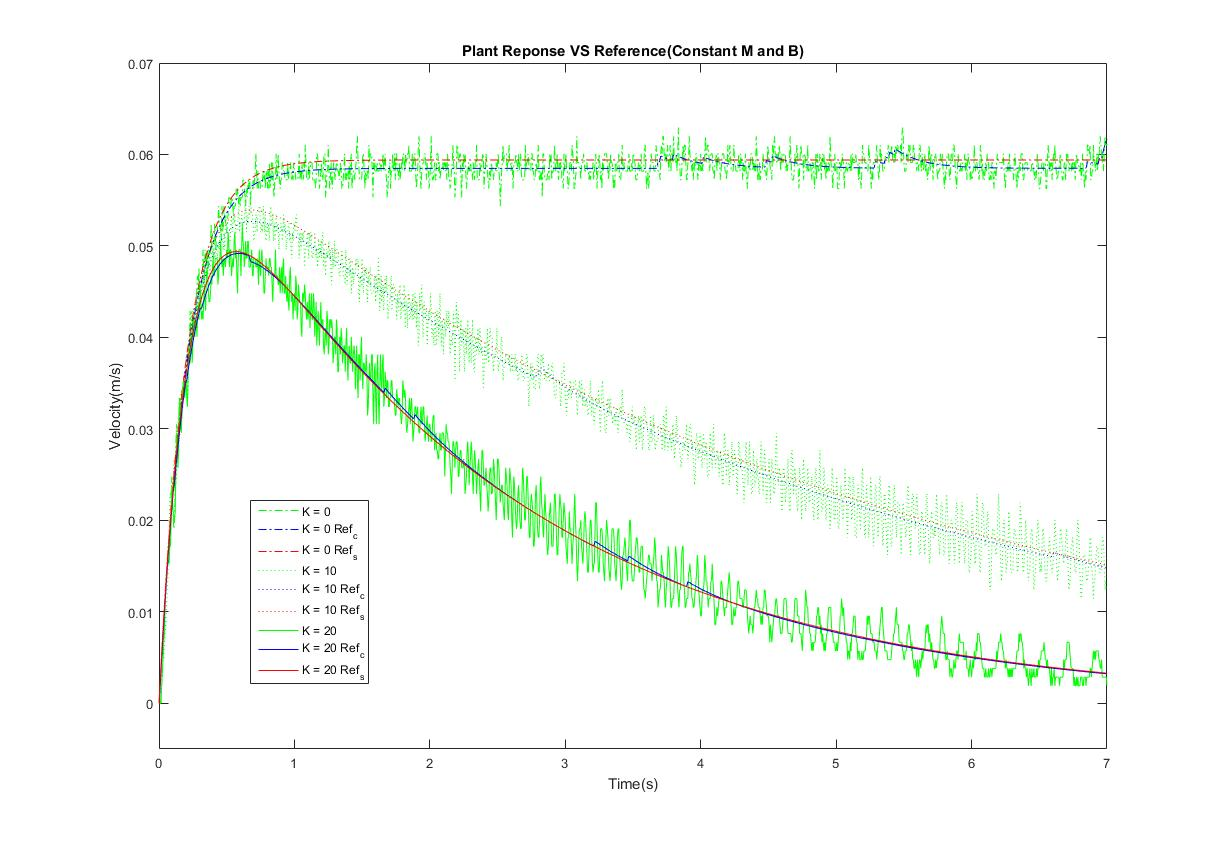
\includegraphics[width=1\linewidth]{Images/KChange}
\caption{Actual and Reference Velocity for Constant Mass and Damping with Adjusted Spring System}
\label{fig:KChange}
\end{figure}

In all three sets, there are significant amount of spikes in recorded velocity, this is mainly due to the small range of speed these tests run at. Since all deviations in speed are on the scale of $10^-3$m/s range, they won't affect overall response. The system is also tested near boundary conditions. The controller is able to handle listed force input for larger force inputs. For smaller force inputs, the noise from load cell and vibration has a stronger effect on reference system which has more potential to cause irregular activity for the motor. Both cases could easily reach the system limit as well thus triggering the warning sound.

After calculating speed error and comparing actual vs. reference response, the controller is determined to be valid and satisfy the design objectives.
